%
\begin{figure}
  \centering
  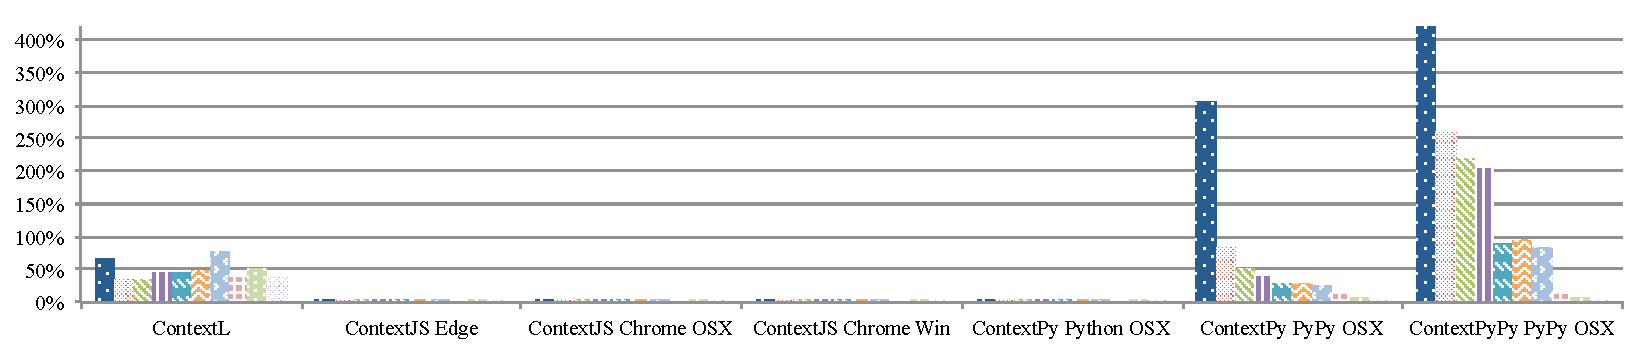
\includegraphics[width=\linewidth]{bench/malte-a/malte-a-1}
  \caption{Bench a overview}
  \label{fig:malte-a-overview}
\end{figure}

%%% Local Variables:
%%% mode: latex
%%% TeX-master: "cop2016-sidewayscomp"
%%% End:

\begingroup
\newcolumntype{P}{S[table-format=3.2]<{{\,\si{\percent}}}}
\begin{table*}[htbp]
\centering
\caption{\copa. Relative throughput of method execution in \protect\acs{cop}
  implementations with 0 to 10 layers normalized to the respective non-layered
  workload. Higher is better.}
\label{tab:copa}
\smaller
\begin{tabular}{@{}rPPPPPPP@{}}
\toprule
 & \multicolumn{1}{c}{ContextL} & \multicolumn{1}{c}{ContextJS} & \multicolumn{1}{c}{ContextJS} & \multicolumn{1}{c}{ContextJS} & \multicolumn{1}{c}{ContextPy} & \multicolumn{1}{c}{ContextPy} & \multicolumn{1}{c}{ContextPyPy}\\
 & \multicolumn{1}{c}{~} & \multicolumn{1}{c}{Edge} & \multicolumn{1}{c}{Chrome OSX} & \multicolumn{1}{c}{Chrome Win} & \multicolumn{1}{c}{Python OSX} & \multicolumn{1}{c}{PyPy OSX} & \multicolumn{1}{c}{PyPy OSX}\\
\midrule
no activate layer & 67.17 & 0.04 & 0.13 & 0.05 & 4.20 & 347.33 & 441.73 \\
1 active layer & 35.90 & 0.09 & 0.09 & 0.03 & 4.11 & 72.76 & 243.82 \\
2 active layer & 36.66 & 0.08 & 0.07 & 0.03 & 3.86 & 47.07 & 244.15 \\
3 active layer & 43.75 & 0.10 & 0.06 & 0.02 & 3.80 & 37.48 & 196.92 \\
4 active layer & 44.90 & 0.08 & 0.05 & 0.04 & 3.65 & 27.90 & 86.65 \\
5 active layer & 47.81 & 0.12 & 0.05 & 0.05 & 3.58 & 28.67 & 94.42 \\
6 active layer & 77.95 & 0.22 & 0.05 & 0.05 & 3.45 & 26.40 & 90.14 \\
7 active layer & 42.77 & 0.18 & 0.06 & 0.05 & 3.42 & 12.38 & 16.06 \\
8 active layer & 49.87 & 0.18 & 0.06 & 0.05 & 3.43 & 5.17 & 5.35 \\
9 active layer & 37.90 & 0.18 & 0.06 & 0.06 & 3.50 & 4.42 & 4.51 \\
\bottomrule
\end{tabular}
\end{table*}
\begin{table*}[htbp]
\centering
\caption{\copb. Relative throughput of layer activation in \protect\acs{cop}
  implementations with 0 to 10 layers normalized to the respective non-layered
  workload. Higher is better.}
\label{tab:copb}
\smaller
\begin{tabular}{@{}rPPPPPPP@{}}
\toprule
 & \multicolumn{1}{c}{ContextL} & \multicolumn{1}{c}{ContextJS} & \multicolumn{1}{c}{ContextJS} & \multicolumn{1}{c}{ContextJS} & \multicolumn{1}{c}{ContextPy} & \multicolumn{1}{c}{ContextPy} & \multicolumn{1}{c}{ContextPyPy}\\
 & \multicolumn{1}{c}{~} & \multicolumn{1}{c}{Edge} & \multicolumn{1}{c}{Chrome OSX} & \multicolumn{1}{c}{Chrome Win} & \multicolumn{1}{c}{Python OSX} & \multicolumn{1}{c}{PyPy OSX} & \multicolumn{1}{c}{PyPy OSX}\\
\midrule
no activate layer & 100.00 & 100.00 & 100.00 & 100.00 & 100.00 & 100.00 & 100.00 \\
1 active layer & 74.97 & 91.56 & 50.00 & 71.13 & 89.22 & 89.59 & 80.16 \\
2 active layer & 66.25 & 67.17 & 50.00 & 52.01 & 80.41 & 61.37 & 21.88 \\
3 active layer & 57.18 & 63.70 & 25.00 & 38.59 & 72.23 & 43.84 & 13.81 \\
4 active layer & 22.56 & 53.07 & 25.00 & 29.40 & 66.51 & 34.79 & 10.32 \\
5 active layer & 24.72 & 45.31 & 12.50 & 22.74 & 61.59 & 30.19 & 8.08 \\
\bottomrule
\end{tabular}
\end{table*}
\endgroup
\clearpage\onecolumn
\begingroup
\newcolumntype{B}{S[table-auto-round = true,exponent-product=\cdot,scientific-notation=true,table-figures-decimal=2,table-figures-integer=2,table-figures-exponent=1]}
\newcolumntype{T}{S[table-auto-round = true,table-format=2.2]}
% % \rotFPtop=0pt plus 1fil
% \rotFPtop=0pt
% \rotFPbot=0pt plus 1fil
\begin{sidewaystable}
\centering
% \begin{table}
\caption{Raw numbers for the comparison benchmarks (\copa \& \copb). \emph{ops} is number of
  operations (higher is better), \emph{time (s)} is time in seconds (lower is
  better), \emph{ops / s} is number of operations per second (higher is
  better).}
\label{tab:copall}
% \begin{sideways}
\smaller\smaller
\sisetup{table-number-alignment = center}
% \hspace*{-1cm}
\begin{tabular}{%
@{}c@{}r@{\enspace}
B@{}T@{}B@{\quad}
B@{}T@{}B@{\quad}
B@{}T@{}B@{\quad}
B@{}T@{}B@{\quad}
B@{}T@{}B@{\quad}
B@{}T@{}B@{\quad}
B@{}T@{}B
@{}}
\toprule
	&&\multicolumn{3}{c}{ContextL}&\multicolumn{3}{c}{ContextJS Edge}&\multicolumn{3}{c}{ContextJS Chrome OSX}&\multicolumn{3}{c}{ContextJS Chrome Win}&\multicolumn{3}{c}{ContextPy Python OSX}&\multicolumn{3}{c}{ContextPy PyPy OSX}&\multicolumn{3}{c}{ContextPyPy PyPy OSX} \\ 
\midrule
	&&{ops }&{ time (s) }&{ ops / s }&{ ops }&{ time (s) }&{ ops / s }&{ ops }&{ time (s) }&{ ops / s }&{ ops }&{ time (s) }&{ ops / s }&{ ops }&{ time (s) }&{ ops / s }&{ ops }&{ time (s) }&{ ops / s }&{ ops }&{ time (s) }& {ops / s} \\ 
\midrule
\parbox[t]{2mm}{\multirow{10}{*}{\rotatebox[origin=c]{90}{NoLayer}}}
 & 1 & 819200000 & 6.963 & 117650438 & 838860800 & 7.719 & 108674802 & 3355443200 & 9.555 & 351171450 & 3355443200 & 9.819 & 341729626 & 25600000 & 5.522 & 4636001 & 819200000 & 8.098 & 101160780 & 819200000 & 8.500 & 96376471 \\
 & 2 & 409600000 & 5.213 & 78572799 & 838860800 & 8.256 & 101606202 & 3355443200 & 9.603 & 349416141 & 1677721600 & 5.108 & 328449804 & 25600000 & 9.092 & 2815662 & 819200000 & 9.166 & 89373773 & 819200000 & 9.036 & 90659584 \\
 & 3 & 409600000 & 6.410 & 63900156 & 838860800 & 8.896 & 94296403 & 3355443200 & 9.590 & 349889802 & 1677721600 & 5.335 & 314474527 & 12800000 & 5.999 & 2133689 & 409600000 & 5.123 & 79953152 & 409600000 & 5.281 & 77561068 \\
 & 4 & 409600000 & 8.351 & 49048018 & 419430400 & 5.796 & 72365493 & 3355443200 & 9.576 & 350401337 & 1677721600 & 5.190 & 323260424 & 12800000 & 7.677 & 1667318 & 409600000 & 5.811 & 70487007 & 409600000 & 5.889 & 69553405 \\
 & 5 & 409600000 & 9.983 & 41029751 & 419430400 & 5.327 & 78736700 & 3355443200 & 9.620 & 348798669 & 1677721600 & 5.859 & 286349479 & 12800000 & 9.036 & 1416556 & 409600000 & 6.614 & 61929241 & 409600000 & 6.542 & 62610822 \\
 & 6 & 204800000 & 5.975 & 34276151 & 419430400 & 9.751 & 43014091 & 1677721600 & 5.238 & 320298129 & 1677721600 & 6.689 & 250818000 & 6400000 & 5.254 & 1218120 & 409600000 & 7.564 & 54151243 & 409600000 & 7.649 & 53549484 \\
 & 7 & 204800000 & 10.780 & 18998145 & 209715200 & 9.131 & 22967386 & 1677721600 & 6.220 & 269730161 & 1677721600 & 8.961 & 187224819 & 6400000 & 5.813 & 1100981 & 409600000 & 8.326 & 49195292 & 409600000 & 8.629 & 47467841 \\
 & 8 & 102400000 & 5.015 & 20418744 & 209715200 & 8.107 & 25868410 & 1677721600 & 6.982 & 240292409 & 1677721600 & 9.384 & 178785337 & 6400000 & 6.586 & 971758 & 409600000 & 9.509 & 43074982 & 409600000 & 9.485 & 43183975 \\
 & 9 & 102400000 & 6.229 & 16439236 & 209715200 & 8.749 & 23970191 & 1677721600 & 8.120 & 206615961 & 838860800 & 5.829 & 143911614 & 6400000 & 7.351 & 870630 & 204800000 & 5.006 & 40910907 & 204800000 & 5.236 & 39113827 \\
 & 10 & 102400000 & 6.189 & 16545484 & 209715200 & 9.537 & 21989640 & 1677721600 & 8.894 & 188635215 & 838860800 & 6.809 & 123198825 & 6400000 & 8.255 & 775288 & 204800000 & 5.325 & 38460094 & 204800000 & 5.467 & 37461130 \\
\midrule
\parbox[t]{2mm}{\multirow{10}{*}{\rotatebox[origin=c]{90}{WithLayer}}}
 & 0 & 409600000 & 5.183 & 79027590 & 409600 & 9.138 & 44824 & 3276800 & 7.003 & 467914 & 3276800 & 17.507 & 187171 & 3200000 & 16.429 & 194778 & 3276800000 & 9.326 & 351361784 & 3276800000 & 7.697 & 425724308 \\
 & 1 & 204800000 & 7.261 & 28205481 & 819200 & 8.575 & 95534 & 1638400 & 5.028 & 325855 & 819200 & 8.145 & 100577 & 3200000 & 27.652 & 115724 & 409600000 & 6.299 & 65026195 & 1638400000 & 7.412 & 221046951 \\
 & 2 & 204800000 & 8.743 & 23424454 & 409600 & 5.346 & 76618 & 1638400 & 6.335 & 258627 & 409600 & 5.001 & 81904 & 3200000 & 38.870 & 82326 & 204800000 & 5.442 & 37633223 & 1638400000 & 8.652 & 189366620 \\
 & 3 & 204800000 & 9.543 & 21460757 & 409600 & 5.764 & 71062 & 1638400 & 7.419 & 220838 & 409600 & 6.088 & 67280 & 3200000 & 50.551 & 63302 & 204800000 & 7.752 & 26418989 & 819200000 & 5.981 & 136967062 \\
 & 4 & 102400000 & 5.558 & 18423893 & 409600 & 6.410 & 63900 & 1638400 & 8.578 & 191000 & 819200 & 6.487 & 126283 & 3200000 & 61.862 & 51728 & 102400000 & 5.927 & 17276869 & 409600000 & 7.550 & 54251656 \\
 & 5 & 102400000 & 6.249 & 16386622 & 409600 & 7.626 & 53711 & 1638400 & 9.930 & 164995 & 819200 & 7.186 & 113999 & 3200000 & 73.462 & 43560 & 102400000 & 6.595 & 15526914 & 409600000 & 8.101 & 50561659 \\
 & 6 & 102400000 & 6.915 & 14808388 & 409600 & 8.141 & 50313 & 819200 & 5.525 & 148271 & 819200 & 8.116 & 100936 & 3200000 & 84.179 & 38014 & 102400000 & 7.883 & 12989978 & 409600000 & 9.573 & 42787005 \\
 & 7 & 102400000 & 11.725 & 8733475 & 409600 & 8.639 & 47413 & 819200 & 6.120 & 133856 & 819200 & 9.040 & 90619 & 3200000 & 96.257 & 33244 & 51200000 & 9.605 & 5330557 & 51200000 & 7.381 & 6936729 \\
 & 8 & 51200000 & 6.245 & 8198559 & 409600 & 9.553 & 42877 & 819200 & 6.610 & 123933 & 409600 & 5.211 & 78603 & 3200000 & 107.120 & 29873 & 12800000 & 6.055 & 2113955 & 12800000 & 6.120 & 2091503 \\
 & 9 & 51200000 & 8.165 & 6270667 & 204800 & 5.246 & 39039 & 819200 & 7.291 & 112358 & 409600 & 5.375 & 76205 & 3200000 & 118.057 & 27106 & 12800000 & 7.537 & 1698288 & 12800000 & 7.584 & 1687764 \\
\midrule
\parbox[t]{2mm}{\multirow{6}{*}{\rotatebox[origin=c]{90}{Activation}}}
 & 0 & 102400000 & 5.668 & 18066337 & 204800 & 9.815 & 20866 & 819200 & 9.050 & 90519 & 409600 & 8.773 & 46689 & 3200000 & 85.011 & 37642 & 102400000 & 6.224 & 16452442 & 409600000 & 5.659 & 72380279 \\
 & 1 & 102400000 & 7.560 & 13544974 & 102400 & 5.360 & 19104 & 409600 & 6.661 & 61492 & 204800 & 6.167 & 33209 & 3200000 & 95.279 & 33586 & 102400000 & 6.947 & 14740176 & 409600000 & 7.060 & 58016997 \\
 & 2 & 102400000 & 8.556 & 11968209 & 102400 & 7.306 & 14016 & 409600 & 9.297 & 44057 & 204800 & 8.434 & 24283 & 3200000 & 105.724 & 30267 & 51200000 & 5.071 & 10096628 & 102400000 & 6.465 & 15839134 \\
 & 3 & 102400000 & 9.913 & 10329870 & 102400 & 7.704 & 13292 & 204800 & 6.355 & 32227 & 102400 & 5.683 & 18019 & 3200000 & 117.698 & 27188 & 51200000 & 7.098 & 7213300 & 102400000 & 10.243 & 9997071 \\
 & 4 & 25600000 & 6.281 & 4075784 & 102400 & 9.248 & 11073 & 204800 & 8.587 & 23850 & 102400 & 7.459 & 13728 & 3200000 & 127.820 & 25035 & 51200000 & 8.944 & 5724508 & 51200000 & 6.855 & 7469001 \\
 & 5 & 51200000 & 11.466 & 4465376 & 51200 & 5.416 & 9453 & 102400 & 5.634 & 18175 & 102400 & 9.643 & 10619 & 3200000 & 138.018 & 23185 & 25600000 & 5.154 & 4967016 & 51200000 & 8.750 & 5851429 \\
\bottomrule
\end{tabular}
% \end{sideways}
% \end{table}
\end{sidewaystable}
\endgroup

%%% Local Variables:
%%% mode: latex
%%% TeX-master: "cop2016-sidewayscomp"
%%% End:
